\documentclass[a4paper, 11pt, dvipdfmx]{jsarticle}
\usepackage[utf8]{inputenc}

\usepackage{graphicx}
\usepackage{hyperref}
\usepackage{bookmark}
\usepackage{fontawesome5}
\usepackage{tcolorbox}
\tcbuselibrary{breakable, listingsutf8}

\usepackage{geometry}
\geometry{left=20mm,right=20mm,top=20mm,bottom=20mm}

\usepackage{chngcntr}
\usepackage{listings}
\usepackage{float} % 追加

\tcbset{
  colframe=black,
  colback=gray!20,
  fonttitle=\bfseries\bfseries,
  sharp corners,
  breakable = true,
  boxrule=0.5mm,
  left=1mm,
  right=1mm,
  top=1mm,
  bottom=1mm,
  enlarge top by=1mm, % Adjust the top margin
  enlarge bottom by=1mm, % Adjust the bottom margin
}
\tcbset{
  terminalstyle/.style={
    colframe=black,
    colback=black,
    coltitle=black,
    colbacktitle=white,
    coltext=white,
    fonttitle=\ttfamily,
    rounded corners=north,
    breakable = false,
    title={\faIcon{terminal} terminal},
  },
  yellow/.style={
    colframe=yellow,
    colback=yellow!10,
    coltitle=black,
    fonttitle=\bfseries,
    title={\faIcon{exclamation-triangle} 注意}
  },
  blue/.style={
    colframe=blue,
    colback=blue!10,
    coltitle=white,
    fonttitle=\bfseries,
    title={\faIcon{info-circle} 情報}
  },
  green/.style={
    colframe=green!80!black,
    colback=green!10,
    coltitle=white,
    fonttitle=\bfseries,
    title={\faIcon{bookmark} 補足説明}
  },
}

\newtcolorbox{terminalbox}[1][]{terminalstyle, #1}
\newtcolorbox{commandbox}[2][]{terminalstyle, title={\faIcon{terminal} #2}, #1}
\newtcolorbox{hosokubox}[2][]{green, title={\faIcon{bookmark} #2}, #1}
% \newtcolorbox{hosokubox}[2][]{green, title={\faIcon{bookmark} #2}, #1}
\newtcolorbox{johobox}[2][]{blue, title={\faIcon{info-circle} #2}, #1}
\newtcolorbox{attentionbox}[2][]{yellow, title={\faIcon{exclamation-triangle} #2}, #1}

\usepackage{titlesec}
\usepackage{tocloft}

% セクション番号の変更
\titleformat{\section}{\normalfont\Large\bfseries}{\thesection 章}{1em}{}
\titleformat{\subsection}{\normalfont\large\bfseries}{\thesection.\arabic{subsection}}{1em}{}
\titleformat{\subsubsection}{\normalfont\normalsize\bfseries}{\thesection.\arabic{subsection}.\arabic{subsubsection}}{1em}{}

\begin{document}

\title{Linuxサーバー構築手順書}
\author{大阪公立大学工業高等専門学校\\
3年 知能情報コース 5番\\
ai10pro
}
\date{\today}
\maketitle\thispagestyle{empty}
\newpage
\tableofcontents

\newpage
\setcounter{section}{-1}

\section{はじめに}
この手順書は、LinuxにてWebサーバーを構築するまでの手順を記載している。ターゲットとしてネットワークやhtmlなどの知識が少しあり、サーバー構築をしてみたいという人や、Linuxというものを触ってみたいという人とする。\\
筆者のLinuxなどの歴としては、本手順書を書いている段階で1年程度である。そのため、初心者にある程度寄り添えるように心がけている。\\
次章から説明や手順を記載しているため実際に手を動かしてもらうと理解が深まると思う。\\
それでは楽しいLinuxのお時間をお過ごしください。
\\\\\\
本書の環境\\
■PC:Gateway NE132-f14p
\begin{itemize}
  \item CPU:Intel Celeron N3060
  \item メモリ:4GB
  \item ストレージ:eMMC 64GB
\end{itemize}
■インストールするOS:Ubuntu 22.04 LTS
\\
本手順書の作成にはTexにおける編集補助としてGitHubCopilotを使用している。\\
また、本書の作成にはVScodeを使用している。\\
\\\\
2025年2月10日

\newpage

\section{Linuxについて}
\subsection{Linuxとは}
Linuxは、UNIX系のオペレーティングシステムの一つであり、オープンソースである。UNIX系のオペレーティングシステムは、多くのサーバーで使用されている。Linuxは、サーバーだけでなく、組み込みシステムやスマートフォン、スーパーコンピュータなど、様々な機器で使用されている。例としてRaspberry Piや近年話題となっているSteam deckなどのポータブルゲーミングデバイスなどもLinuxをベースOSにしている。
\subsection{Linuxディストリビューション}
Linuxは、様々なディストリビューションが存在する。ディストリビューションとは、Linuxカーネルに、シェル、コマンド、ライブラリ、デスクトップ環境、アプリケーションなどを組み合わせたものである。代表的なものとして、Ubuntu、Debian、CentOS、Raspberry Pi OSなどがある。\\
本書ではUbuntuの環境を前提として説明を行う。
\subsubsection{カーネル}
Linuxのカーネルは、Linuxの中核となる部分であり、ハードウェアとソフトウェアの間のインターフェースを提供する。カーネルは、プロセス管理、メモリ管理、ファイルシステム、デバイスドライバなどの機能を提供する。
\subsubsection{シェル}
シェルは、ユーザーとカーネルの間のインターフェースを提供する。シェルは、ユーザーがコマンドを入力し、カーネルに命令を伝える。代表的なシェルとして、bash、zsh、fishなどがある。
\subsubsection{コマンド}
シェルを通して実行するプログラムであり、Linuxには数千にもなるコマンドが存在するが基本的に使用する物は限られているためサーバー運用においては覚えておくことで作業効率が向上する。
\subsubsection{ライブラリ}
ライブラリは、プログラムの共通部分をまとめたものであり、プログラムの開発を効率化する。ライブラリは、プログラムの実行時にリンクされる。
\subsection{ファイルやディレクトリ構造について}
Linuxではディレクトリ構造がWindowsとは異なる。
\subsubsection{ファイルの種類}
  Linuxで扱われるファイルは以下のように分類される。
  \begin{itemize}
    \item ファイル     :テキストファイルとバイナリファイル
    \item リンクファイル :シンボリックリンクとハードリンク
    \item 特殊ファイル  :デバイスファイルや隠しファイル
    \item ディレクトリ  :ファイルを集約するためのWindowsでいうフォルダ
  \end{itemize}
  拡張子はWindowsにおいてはアプリケーションの起動に紐づけられていたが、Linuxでは単なるファイル名の一部として認識される。\\
  Linuxではデバイスファイルがあり、これはハードウェアをファイルとして扱うためのものである。\\

  \subsubsection{ディレクトリ構造}
  Linuxのディレクトリ構造は/(ルート)を起点として以下のディレクトリが主に挙げられる。それらをある程度理解しておくことで各種設定などの変更の際に便利である。\\
  表\ref{tab:directories}に主要なディレクトリとその説明を示す。
  \begin{table}[H]
    \centering
    \begin{tabular}{|l|l|}
      \hline
      ディレクトリ & 説明 \\ \hline
      /root & システム管理者のホームディレクトリ \\ \hline
      /home & 一般ユーザーのホームディレクトリ \\ \hline
      /bin & 一般ユーザーでも実行可能なコマンドが含まれるディレクトリ \\ \hline
      /sbin & sudo権限またはroot権限が必要なコマンドが含まれるディレクトリ \\ \hline
      /media & USBメモリや外付けHDDなどのデバイスがマウントされるディレクトリ \\ \hline
      /etc & システムの設定ファイルが含まれるディレクトリ \\ \hline
      /usr & システム全体で共有されるアプリケーション、ライブラリ、ドキュメントなどが保存されるディレクトリ \\ \hline
      /lib & ライブラリが保存されるディレクトリ \\ \hline
      /proc & カーネルやプロセスに関する情報が保存されるディレクトリ \\ \hline
      /tmp & 一時ファイルが保存されるディレクトリ \\ \hline
      /var & 変化するデータが保存されるディレクトリ、ログファイルやデータベースなど \\ \hline
    \end{tabular}
    \caption{主要なディレクトリとその説明}
    \label{tab:directories}
  \end{table}


\section{Ubuntuインストール}
\subsection{Ubuntuとは}
Ubuntuは、Linuxディストリビューションの一つであり、デスクトップ環境を提供する。また、サーバー版も提供されており、サーバー運用にも使用される。Ubuntuは、Debianをベースにしており、Debianの安定性とUbuntuの使いやすさを兼ね備えている。また、Ubuntuは、オープンソースであり、無料で利用することができる。\\
\subsection{インストール環境}
  本書の環境を再度記載する。\\
  ■PC:Gateway NE132-f14p
  \begin{itemize}
    \item CPU:Intel Celeron N3060
    \item メモリ:4GB
    \item ストレージ:eMMC 64GB
  \end{itemize}
  ■インストールするOS:Ubuntu 22.04 LTS
  \begin{johobox}{最新版Ubuntu}
    最新のUbuntuのバージョンは24.04 LTSである。しかし、本書では22.04 LTSを使用する。理由として、ドキュメントが豊富であり、安定しているためである。最新バージョンと22.04 LTSでは一部UIが違う部分もあるため、注意が必要である。
  \end{johobox}
\subsection{インストールメディアの準備}
  \begin{enumerate}
    \item UbuntuのISOファイルをダウンロード
    \begin{tcolorbox}[blue]
      Ubuntu を入手する \href{https://releases.ubuntu.com/20.04/}{\texttt{https://releases.ubuntu.com/20.04/}}\\
      Ubuntu Desktop 日本語 Remixのダウンロード \href{https://www.ubuntulinux.jp/download/ja-remix}{\texttt{https://www.ubuntulinux.jp/download/ja-remix}}
    \end{tcolorbox}
    \item Rufusをダウンロード
    \begin{tcolorbox}[blue]
      Rufusを入手する \href{https://rufus.ie/ja/}{\texttt{https://rufus.ie/ja/}}
    \end{tcolorbox}
    \item Rufusを起動し、デバイス、ブート選択、イメージ選択を行う\\
    デバイスにはインストールメディアとするためのUSBを選択する。\\
    ブート選択では、先ほどダウンロードしたISOファイルを選択する。\\
    パーティション構成は一般的にはMBRでよい。ただし、Gatewayの場合はGPTを選択する。その他の設定はデフォルトのままでよい。
      \begin{tcolorbox}[yellow]
        デバイスを選択する際は注意が必要である。間違えるとPCや外部ストレージのデータが消える可能性があるため、注意が必要である。
      \end{tcolorbox}
    \item スタートをクリックし、書き込みを開始する
  \end{enumerate}

\subsection{Boot Modeの変更}
  \begin{enumerate}
    \item 電源をつけF2を連打しBIOS画面を表示
    \begin{hosokubox}{BIOS画面の操作}
      BIOS画面は基本的にキーボードで操作されることが多い。一部メーカーの場合はマウスで操作することもあるが、基本的にはキーボードでの操作が必要である。
    \end{hosokubox}
    \item Securityに移動しSupervisor Passwordを設定\\
    一度Enterを押し、パスワードを入力し、再度Enterを押し、もう一度パスワードを入力し、Enterを押す。\\
    \item Bootに移動しBoot ModeをLegacyに変更
    \item F10で保存して再起動
    \item F2を連打しBIOS画面を表示
    \item Bootに移動しBoot Priorityを変更しインストールメディアが入るものを選択\\
    作成したインストールメディアを選択する。選択にはF5またはF6を使用し順番を変更する。\\
    \item Boot ModeをUEFIに変更
    \item SecureBootをDisableに変更
    \item F10で保存して再起動
  \end{enumerate}
\subsection{Ubuntuのインストール}
  \begin{enumerate}
    \item 再起動後自動的にBoot Menuが表示される
    \item Try or Install Ubuntuを選択
    % \item 以下Ubuntuのインストールを書く ★
    \item インストールの種類を選択
    \item インストール先を選択
    \item キーボードレイアウトを選択
    \item ユーザー情報を入力
    \item インストールが完了したら再起動
  \end{enumerate}
\subsection{インストール後の再起動}
  \begin{enumerate}
    \item 再起動時にBiosに入る
    \item Bootに移動しBoot Priorityを変更しインストールしたディスクを1番目にする
    \item SecureをEnableに変更
    \item Securityに移動しErase all Secure Boot Settingを選択し、Boot設定を削除
    \item Select an UEFI file as trusted for executingを選択
    \item EMMC \textgreater EFI \textgreater Ubuntu \textgreater shimx64.efiを選択
    \item Boot名を入力し、Enter
    \item Bootに移動しSecure BootをDisableに変更
    \item Securityに移動しSupervisor Passwordを削除\\
    Supervisor PasswordにてEnterを押し、今のパスワードを入力、Enterを押し、何も入力しないままEnterを押す、もう一度行うことでパスワードが削除される。
    \item F10で保存して再起動
    \item ログイン画面になったら成功
  \end{enumerate}

\section{Ubuntuの各種設定・インストール}
Ubuntu(Linux)はWindowsなどと同様に様々な設定が可能である。以下にはその一部を示すが、適宜自分にあったUbuntu環境を構築することが望ましい。練習ついでにいろいろな物を入れてみるとよい。
\subsection{日本語入力}
  Ubuntuではデフォルトでキーボードによる日本語入力は対応していない。そのため、以下の手順で日本語入力を可能にする。なお日本語入力には一般に「Mozc」が使用されることが多い。
  \begin{enumerate}
    \item ターミナルを開く
    \item 以下のコマンドを実行
    \begin{terminalbox}
      \verb|$ sudo apt update|\\
      \verb|$ sudo apt install ibus-mozc|
    \end{terminalbox}
    \item 設定 \textgreater キーボード \textgreater 入力ソース \textgreater 日本語(Mozc)を追加
    \item Windowsキー + Spaceで日本語入力が可能になる\\
    なお、右上にある「A」をクリックすることで入力ソースを切り替えることができる。
  \end{enumerate}

\subsection{Vimのインストール}
  VimはLinux環境で使用されるテキストエディタであり、非常に高機能である。特徴として、ターミナル上で操作するため、マウスを使わずに編集を行う。本手手順書ではsudo権限(後の章にて解説)の必要なファイルの編集などで使用する。標準で搭載されている場合もある。
  \begin{enumerate}
    \item ターミナルを開く
    \item 以下のコマンドを実行
    \begin{terminalbox}
      \verb|$ sudo apt update|\\
      \verb|$ sudo apt install vim|
    \end{terminalbox}
    \item インストールが完了したら、以下コマンドを実行しインストールされているか確認
    \begin{terminalbox}
      \verb|$ vim --version|
    \end{terminalbox}
  \end{enumerate}

\subsection{VSCodeのインストール}
  VSCodeはMicrosoftが提供するオープンソースのコードエディタであり、非常に高機能である。特徴として、拡張機能を追加することで、様々な言語に対応することができる。また、リモート開発機能を使用することで、リモートサーバー上での開発も可能である。
  \begin{enumerate}
    \item \href{https://code.visualstudio.com/}{\texttt{https://code.visualstudio.com/}}にアクセスし、ダウンロード
    \item ダウンロードしたファイルを開く
    \item インストールを開始
    \item インストールが完了したら、VSCodeを起動
  \end{enumerate}

\subsection{slのインストール(お遊び)} 
  slは、タイプミスでよく入力される「ls」コマンドを実行すると、蒸気機関車が走るアニメーションが表示されるコマンドである。インストールの練習として入れてみるとよい。
  \begin{enumerate}
    \item ターミナルを開く
    \item 以下のコマンドを実行
    \begin{terminalbox}
      \verb|$ sudo apt update|\\
      \verb|$ sudo apt install sl|
    \end{terminalbox}
    \item 以下のコマンドを実行
    \begin{terminalbox}
      \verb|$ sl|
    \end{terminalbox}
  \end{enumerate}
  \begin{figure}[H]
    \centering
    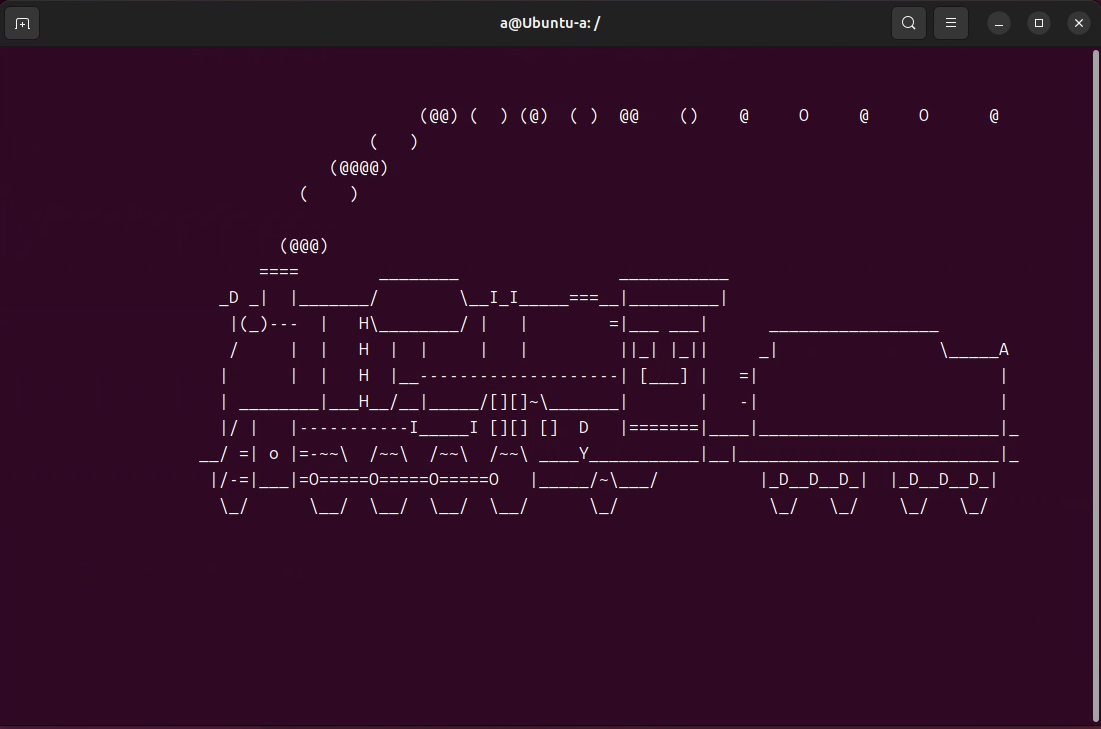
\includegraphics[width=0.5\textwidth]{images/linux-server/3_4-sl.png}
    \caption{slの実行結果}
    \label{fig:sl}
  \end{figure}
  実行時にオプションがあるので、気が向いたら調べて遊んでみるとよい。

\subsection{cmatrixのインストール(お遊び)}
  cmatrixは、映画「マトリックス」に登場するコードのような文字列が画面上を流れるアニメーションを表示するコマンドである。ハッカーみたいになれるのでなりたい人は入れるとよい。
  \begin{enumerate}
    \item ターミナルを開く
    \item 以下のコマンドを実行
    \begin{terminalbox}
      \verb|$ sudo apt update|\\
      \verb|$ sudo apt install cmatrix|
    \end{terminalbox}
    \item 以下のコマンドを実行
    \begin{terminalbox}
      \verb|$ cmatrix|
    \end{terminalbox}
  \end{enumerate}
  \begin{figure}[H]
    \centering
    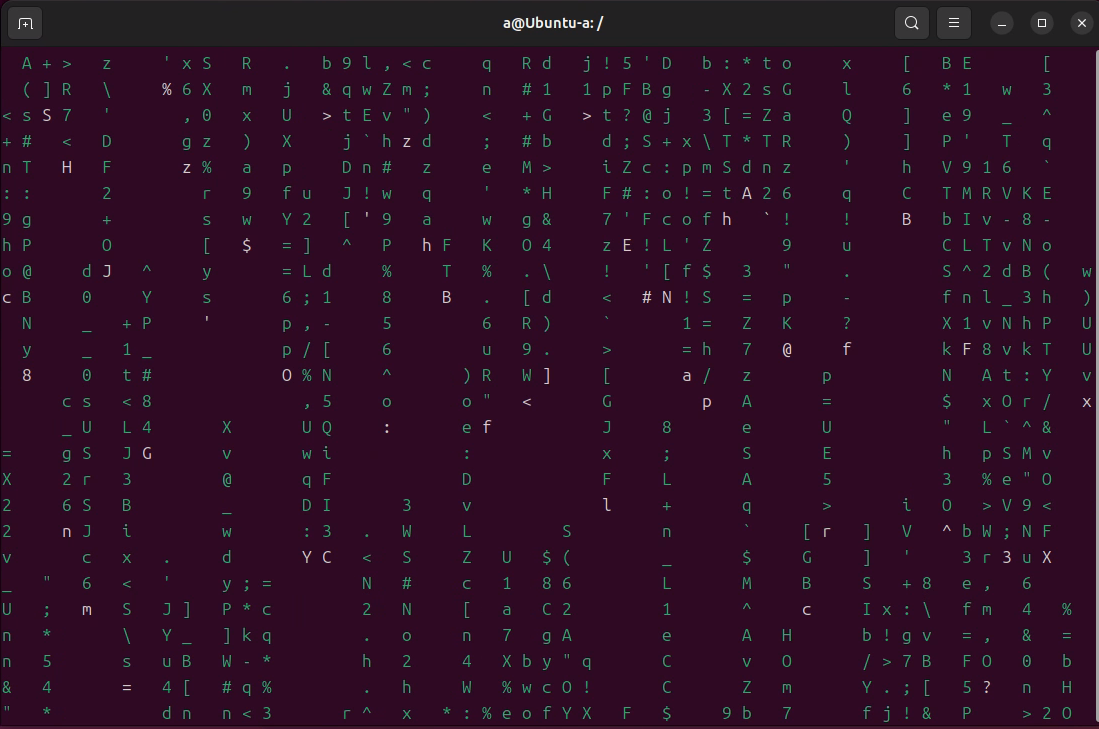
\includegraphics[width=0.5\textwidth]{images/linux-server/3_5-cmatrix.png}
    \caption{cmatrixの実行結果}
    \label{fig:cmatrix}
  \end{figure}

\section{Linuxの基本コマンド}
サーバー上でのシステム操作は一般的にターミナルを用いてコマンド入力により操作を行うことが多い。この章ではLinuxの基本コマンドとして紹介するが、一部コマンドはWindowsでも使用できる。ただし、WindowsのコマンドはLinuxとは異なるため注意が必要である。\\
  コマンドは一般的に以下のように入力する。
\begin{commandbox}{コマンドの入力方法}
  \verb|$ {コマンド名} {オプション} {引数}|
\end{commandbox}

\subsection{よく使うコマンド一覧}
\subsubsection{ファイルやディレクトリの操作}
\begin{itemize}
  \item ls : ファイルやディレクトリの一覧を表示する\\
  オプションなしの場合、カレントディレクトリのファイルやディレクトリの一覧を表示する。
  \begin{terminalbox}
    \verb|$ ls|
    \verb|bin |
  \end{terminalbox}
  \begin{hosokubox}{lsコマンドのオプション}
    -a : 隠しファイルも表示する\\
    -l : 詳細情報を表示する(パーミッション情報)\\
    -h : ファイルサイズを見やすい形式で表示する
  \end{hosokubox}
  \item cd : カレントディレクトリを移動する\\
  ディレクトリ名の場所にカレントディレクトリを移動する。
  \begin{terminalbox}
    \verb|$ cd {ディレクトリ名}|\\\\
    \verb|# ルートディレクトリへの移動|\\
    \verb|$ cd /|
  \end{terminalbox}
  \item pwd : 現在のディレクトリのパスを表示する
  \begin{terminalbox}
    \verb|$ pwd|\\\\
    \verb|例:/homeでの実行結果|\\
    \verb|/home|
  \end{terminalbox}
  \item mkdir : ディレクトリを作成する\\
  pathに指定したディレクトリを作成する。
  \begin{terminalbox}
    \verb|$ mkdir {ディレクトリ名}|\\\\
    \verb|例:testディレクトリを作成する|\\
    \verb|$ mkdir test|
  \end{terminalbox}
  \item rm : ファイルやディレクトリを削除する\\
  一部ファイルはsudo権限が必要である。
  \begin{terminalbox}
    \verb|$ rm {ファイル名}|\\\\
    \verb|例:test.txtを削除する|\\
    \verb|$ rm test.txt|
  \end{terminalbox}
  \item rmdir : ディレクトリを削除する\\
  ディレクトリ内にファイルがある場合は削除できない。
  \begin{terminalbox}
    \verb|$ rmdir {ディレクトリ名}|\\\\
    \verb|例:testディレクトリを削除する|\\
    \verb|$ rmdir test|
  \end{terminalbox}
  \item cp : ファイルやディレクトリをコピーする\\
  copyであるため元のファイルは残る。
  \begin{terminalbox}
    \verb|$ cp {コピー元} {コピー先}|\\\\
    \verb|例:test.txtをtest2.txtにコピーする|\\
    \verb|$ cp test.txt test2.txt|
  \end{terminalbox}
  \item mv : ファイルやディレクトリを移動する\\
  moveであるため元のファイルは消える。
  \begin{terminalbox}
    \verb|$ mv {移動元} {移動先}|\\\\
    \verb|例:test.txtをtest2.txtに移動する|\\
    \verb|$ mv test.txt test2.txt|
  \end{terminalbox}
  \item find : ファイルを検索する
  \begin{terminalbox}
    \verb|$ find {検索先} -name {検索ファイル名}|
  \end{terminalbox}
  \item touch : ファイルを作成する
  \begin{terminalbox}
    \verb|$ touch {ファイル名}|\\\\
    \verb|例:test.txtファイルを作成する|\\
    \verb|$ touch test.txt|
  \end{terminalbox}
  \item ln:シンボリックリンクの作成\\
  ファイルやディレクトリに対してシンボリックリンクを作成する。シンボリックリンクとはWindowsにおけるショートカットの役割を果たすものである。
  \begin{terminalbox}
    \verb|$ ln -s {リンク元} {リンク先}|\\\\
    \verb|例:test.txtのシンボリックリンクをデスクトップに作成する|\\
    \verb|$ ln -s test.txt ~/Desktop/test.txt|
  \end{terminalbox}
\end{itemize}

\subsubsection{テキスト操作}
\begin{itemize}
  \item cat : ファイルの内容を表示する\\
  ファイルの内容をターミナル上でスクロールする形で表示する。
  \begin{terminalbox}
    \verb|$ cat {ファイル名}|
  \end{terminalbox}
  \item less : ファイルの内容をページ単位で表示する
  スペースキーで次のページ、qキーで終了する。
  \begin{terminalbox}
    \verb|$ less {ファイル名}|
  \end{terminalbox}
  \item head : ファイルの先頭部分を表示する\\
  ファイルの先頭部分を表示する。
  \begin{terminalbox}
    \verb|$ head {ファイル名}|
  \end{terminalbox}
  \item tail : ファイルの末尾部分を表示する\\
  ファイルの末尾部分を表示する。
  \begin{terminalbox}
    \verb|$ tail {ファイル名}|
  \end{terminalbox}
  \item grep : ファイル内の文字列を検索する\\
  ファイル内の文字列を検索する。
  \begin{terminalbox}
    \verb|$ grep {検索文字列} {ファイル名}|\\\\
    \verb|例:test.txt内に「test」が含まれているか検索する|\\
    \verb|$ grep test test.txt|
  \end{terminalbox}
  \item vi : Vim(テキストエディタ)の起動\\
  Vimの使用方法については後述する。
  \begin{terminalbox}
    \verb|$ vi {ファイル名}|\\\\
    \verb|例:test.txtを編集する|\\
    \verb|$ vi test.txt|
  \end{terminalbox}
  \item code : VSCode(テキストエディタ)の起動\\
  ファイル名の部分にはディレクトリも指定できる。その場合、そのディレクトリがVSCodeで開かれる。
  \begin{terminalbox}
    \verb|$ code {ファイル名}|\\\\
    \verb|例:test.txtを編集する|\\
    \verb|$ code test.txt|
  \end{terminalbox}
\end{itemize}

\subsubsection{パーミッションや所有者}
\begin{itemize}
  \item chmod : ファイルやディレクトリのパーミッションを変更する\\
  \begin{terminalbox}
    \verb|$ chmod {パーミッション} {ファイル名}|\\\\
    \verb|例:test.txtのパーミッションをrwxr-xr--に変更する|\\
    \verb|$ chmod 754 test.txt|
  \end{terminalbox}
  パーミッションはrwxrwxrwxの形式で表される。rは読み取り、wは書き込み、xは実行を表す。\\
  例えば、rwxr-xr--は所有者に読み取り、書き込み、実行権限があり、グループに読み取り、実行権限があり、その他に読み取り権限があることを示す。
  \begin{hosokubox}{パーミッションの指定方法について}
    パーミッションは数字で指定することができる。\\
    rwx/rwx/rwxという風に3桁ごとに区切って考える。rを4, wを2, xを1として、それぞれの権限を足し合わせる。したがって、rwxr-xr--は754と表すことができる。\\
    ※この数字は2進数で処理しており、rwxの時111となり、合計が7となる。
  \end{hosokubox}
  \item chown : ファイルやディレクトリの所有者を変更する
  \begin{terminalbox}
    \verb|$ chown {所有者}:{グループ} {ファイル名}|\\\\
    \verb|例:test.txtの所有者をrootに変更する|\\
    \verb|$ chown root test.txt|
  \end{terminalbox}
  グループ名は省略することもできる。その場合、所有者と同じグループになる。
  \item chgrp : ファイルやディレクトリのグループを変更する
  \begin{terminalbox}
    \verb|$ chgrp {グループ} {ファイル名}|\\\\
    \verb|例:test.txtのグループをrootに変更する|\\
    \verb|$ chgrp root test.txt|
  \end{terminalbox}
\end{itemize}

\subsubsection{ネットワーク管理}
\begin{itemize}
  \item ping : ネットワークの接続確認を行う
  \begin{terminalbox}
    \verb|$ ping {IPアドレス}|\\\\
    \verb|例:192.168.0.150にpingを送信する|\\
    \verb|$ ping 192.168.0.150|
  \end{terminalbox}
  \begin{hosokubox}{pingコマンドについて}
    pingコマンドはネットワーク内の機器の接続確認でよく使用される。Windowsでも同様に使用できる。ただし、Windowsは4回の送信で終了するが、LinuxはCtrl + Cで終了するまで続く。
  \end{hosokubox}
  \begin{hosokubox}{pingコマンドのオプション}
    -c : 指定回数の送信を行う\\
    -i : 送信間隔を指定する\\
    -t : 継続的に送信を行う
  \end{hosokubox}
  \item ifconfig : ネットワークインターフェースの情報を表示する
  \begin{terminalbox}
    \verb|$ ifconfig|
  \end{terminalbox}
  出力例は以下の通りである。
  \begin{figure}[H]
    \centering
    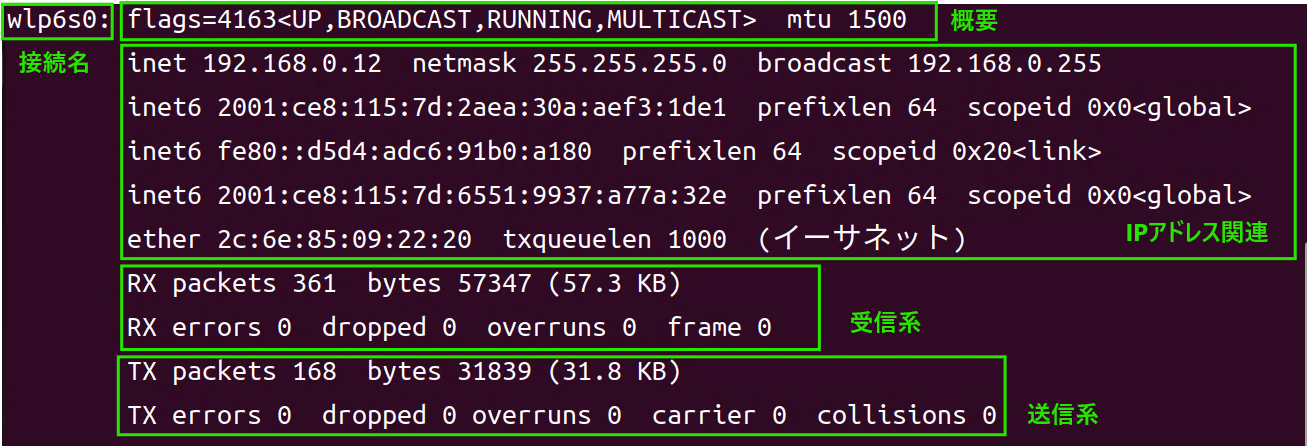
\includegraphics[width=0.8\textwidth]{images/linux-server/4_1_4-1-ifconfig.png}
    \caption{ifconfigの出力例}
    \label{fig:your_image}
  \end{figure}
  各種いろいろなネットワークアダプタに関する情報を取得できるがため調べて利用するとよい。ただし、IPアドレス関連にあるinetアドレスは、IPv4のアドレスでありよく使うため覚えておくとよい。
  \item route : ルーティングテーブルの情報を表示する
  \begin{johobox}{ルーティングとは}
    ルーティングとは、ネットワーク上のデータを送信する際に、どの経路を通って送信するかを決定することである。ルーティングテーブルは、どの経路を通って送信するかを示すものである。
  \end{johobox}
  \begin{terminalbox}
    \verb|$ route|
  \end{terminalbox}
  \item netstat : ネットワークの接続状況を表示する
  \begin{terminalbox}
    \verb|$ netstat|\\\\
    \verb|例:全ての接続状況を表示する|\\
    \verb|$ netstat -a|
  \end{terminalbox}
  \begin{hosokubox}{netstatコマンドのオプション}
    -a : 全ての接続状況を表示する\\
    -t : TCP接続のみを表示する\\
    -u : UDP接続のみを表示する\\
    -n : IPアドレスを表示する
  \end{hosokubox}
  \item ssh : リモートサーバーに接続する\\
  詳細については10章で解説する。
  \begin{terminalbox}
    \verb|$ ssh {ユーザー名}@{IPアドレス}|
  \end{terminalbox}
  \item ftp : ファイル転送プロトコルを使用してファイルを転送する
  \begin{terminalbox}
    \verb|$ ftp {IPアドレス}|
  \end{terminalbox}
\end{itemize}

\subsubsection{システム管理}
\begin{itemize}
  \item top : システムのリソース使用状況を表示する
  \begin{terminalbox}
    \verb|$ top|
  \end{terminalbox}
  \begin{hosokubox}{topコマンドの操作方法}
    q : 終了する\\
    P : CPU使用率でソートする\\
    M : メモリ使用率でソートする\\
    T : 実行時間でソートする
  \end{hosokubox}
  \item ps : 現在実行中のプロセスの情報を表示する
  \begin{terminalbox}
    \verb|$ ps|\\\\
    \verb|例:全てのプロセスを表示する|\\
    \verb|$ ps -ef|
  \end{terminalbox}
  \begin{hosokubox}{psコマンドのオプション}
    -e : 全てのプロセスを表示する\\
    -f : 詳細情報を表示する
  \end{hosokubox}
  \item kill : プロセスを終了する
  \begin{terminalbox}
    \verb|$ kill {プロセスID}|\\\\
    \verb|例:プロセスIDが1234のプロセスを終了する|\\
    \verb|$ kill 1234|
  \end{terminalbox}
  \item df : ディスクの使用状況を表示する
  \begin{terminalbox}
    \verb|$ df|
  \end{terminalbox}
  \item du : ディレクトリのディスク使用量を表示する
  \begin{terminalbox}
    \verb|$ du {ディレクトリ名}|\\\\
    \verb|例:testディレクトリのディスク使用量を表示する|\\
    \verb|$ du test|
  \end{terminalbox}
  \item free : メモリの使用状況を表示する
  \begin{terminalbox}
    \verb|$ free|
  \end{terminalbox}
  \item uptime : システムの稼働時間を表示する
  \begin{terminalbox}
    \verb|$ uptime|
  \end{terminalbox}
  \item uname : システム情報を表示する
  \begin{terminalbox}
    \verb|$ uname|\\\\
    \verb|例:システム情報を表示する|\\
    \verb|$ uname -a|
  \end{terminalbox}
  \begin{hosokubox}{unameコマンドのオプション}
    -a : 全ての情報を表示する\\
    -s : カーネル名を表示する\\
    -r : カーネルリリースを表示する\\
    -v : カーネルバージョンを表示する\\
    -m : マシンハードウェアを表示する
  \end{hosokubox}
\end{itemize}

\subsubsection{ユーザー管理}
以下コマンドはsudo権限が必要である。\\
各コマンドの詳細は後述する。
\begin{itemize}
  \item useradd / adduser : ユーザーの新規作成
  \item passwd : パスワードの変更
  \item usermod / chfn : ユーザー情報の変更
  \item userdel : ユーザーの削除
  \item groupadd : グループの新規作成
  \item who : ログイン中のユーザーを表示する
\end{itemize}

\subsection{シェルに備わっている機能}
シェルには様々な機能が備わっており、これらを使用することで作業効率を向上させることができる。以下に代表的な機能を紹介する。
\subsubsection{入力補完}
入力補完は、コマンドやファイル名の入力時にTabキーを押すことで、入力を補完する機能である。入力補完を使用することで、入力ミスを防ぐことができる。使用方法は入力中にTabキーを押すだけである。ただし、複数の候補がある場合はTabキーを押しても補完されない場合がある。その場合はTabキーを2回押すことで候補が表示される。
\subsubsection{コマンド履歴}
コマンド履歴は、過去に入力したコマンドを表示する機能である。矢印キーを使用することで、過去に入力したコマンドを表示することができる。矢印キーの上を押すことで過去のコマンドを表示し、矢印キーの下を押すことで新しいコマンドを表示することができる。
\begin{hosokubox}{インクリメンタル検索}
  Ctrl + Rを押すことで、過去に入力したコマンドを検索することができる。過去に入力したコマンドを検索し下矢印キーを押すことで検索したコマンドを入力することができる。
\end{hosokubox}

\subsubsection{パイプとリダイレクト}
Linuxでコマンド入力をする際複数コマンドを組み合わせたい時がある。それらを組み合わせる際に使用するのがパイプである。パイプは「\textbar」を使用してコマンドをつなげることで、前のコマンドの出力を次のコマンドの入力として使用することができる。\\
  \begin{terminalbox}
    \verb|$ {コマンド1} | \textbar{} \verb| {コマンド2}|\\\\
    例:lsコマンドの出力をgrepコマンドに渡してtestを検索する\\
    \verb|$ ls | \textbar{} \verb| grep test|
  \end{terminalbox}
また、実行したコマンドの出力をファイルに保存することができる。これをリダイレクトという。リダイレクトは「\textgreater」を使用して出力をファイルに保存することができる。\\
\begin{terminalbox}
  \verb|$ {コマンド} > {ファイル名}|\\\\
  例:lsコマンドの出力をtest.txtに保存する\\
  \verb|$ ls > test.txt|
\end{terminalbox}
\begin{hosokubox}{上書きと追記}
  リダイレクトする際、ファイルが存在する場合は上書きされる。ファイルの内容を保持したまま追記したい場合は「\textgreater\textgreater」を使用する。
\end{hosokubox}
\section{パーミッション}
\subsection{ファイルの所有者}
Linuxではファイルやディレクトリに所有者が設定されている。所有者はファイルやディレクトリを作成したユーザーであり、所有者はファイルやディレクトリに対して権限を持っている。所有者はユーザー名で表される。\\
実際に確認するには、lsコマンドに「-l」オプションを付けて実行する。実行結果は以下のようになる。
\begin{figure}[H]
  \centering
  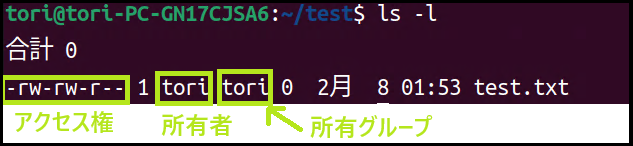
\includegraphics[width=0.8\textwidth]{images/linux-server/5_1-ls-l.png}
  \caption{ls -lの実行結果}
  \label{fig:ls-l}
\end{figure}
\subsection{アクセス権}
Linuxではファイルやディレクトリに対してアクセス権が設定されている。アクセス権は読み取り、書き込み、実行の3つの権限が設定されている。アクセス権は所有者、グループ、その他の3つに設定されている。\\
\begin{hosokubox}{ファイルのアクセス権}
  \begin{itemize}
    \item r : 読み取り権限  ファイルの内容を読み取ることができる
    \item w : 書き込み権限  ファイルの内容を書き込むことができる
    \item x : 実行権限  ファイルを実行することができる
  \end{itemize}
\end{hosokubox}
\begin{hosokubox}{ディレクトリのアクセス権}
  \begin{itemize}
    \item r : 読み取り権限  ディレクトリ内のファイルを表示することができる
    \item w : 書き込み権限  ディレクトリ内にファイルを作成することができる
    \item x : 実行権限  ディレクトリ内に移動することができる
  \end{itemize}
\end{hosokubox}
\begin{johobox}{ls -lで表示される種類について}
  ls -lで表示される先頭の文字はファイルの種類を示している。以下に一部を示す。
  \begin{itemize}
    \item \verb|- : 通常のファイル|
    \item \verb|d : ディレクトリ|
    \item \verb|l : シンボリックリンク|
  \end{itemize}
\end{johobox}
\subsection{パーミッションの変更}
アクセス権の変更にはchmodコマンドを使用する。ただし、アクセス権の変更にはsodo権限が必要である。\\
\begin{commandbox}{chmodコマンドの使用方法}
  \verb|chmod {パーミッション} {ファイル名}|\\
  \verb|chmod {パーミッション} {ディレクトリ名}|
\end{commandbox}
また、アクセス権の変更には記号を用いた方法と数値を用いた方法がある。数値を用いたものは前述しているため、ここでは記号を用いた方法について説明する。
\begin{table}[H]
  \centering
  \caption{chmodコマンドの記号について}
  \begin{tabular}{|c|c|c|} \hline
    対象 & 操作 & 権限 \\ \hline
    u:所有者 & +:追加 & r:読み取り権限 \\
    g:所有グループ & -:削除 & w:書き込み権限 \\
    o:その他ユーザー & =:指定 & x:実行権限 \\
    a:全てのユーザー & & \\ \hline
  \end{tabular}
\end{table}
\begin{hosokubox}{chmodコマンドの使用例}
  \begin{itemize}
    \item \verb|chmod u+x test.txt| : test.txtに所有者に実行権限を追加する
    \item \verb|chmod g-w test.txt| : test.txtに所有グループから書き込み権限を削除する
    \item \verb|chmod o=r test.txt| : test.txtにその他ユーザーに読み取り権限を指定する
    \item \verb|chmod a=rwx test.txt| : test.txtに全てのユーザーに読み取り、書き込み、実行権限を指定する
  \end{itemize}
\end{hosokubox}
\subsection{所有者と所有グループ}
Linuxにおけるファイルやディレクトリは作成したユーザーが所有者・所有グループとなる。しかし、一定以上のサーバー管理となる場合、管理体系などの理由により管理者レベルの高いユーザーに所有権を譲渡する必要がある。その際にchownコマンドを使用する。
\begin{commandbox}{chownコマンドの使用方法}
  \verb|chown {所有者} {ファイル名(ディレクトリ名)}|\\
  \verb|chgrp {所有グループ} {ファイル名(ディレクトリ名)}|
\end{commandbox}
\begin{attentionbox}{chownコマンドの注意点}
  chownコマンドはsudo権限が必要である。また、ファイルやディレクトリの所有者を変更する際は、そのファイルやディレクトリに対して所有者権限を持っている必要がある。
\end{attentionbox}
\section{環境変数}
環境変数は、システム全体で使用される変数である。環境変数はシェルが起動する際に設定され、シェルの終了時に破棄される。環境変数はシェルスクリプトやプログラムから参照することができる。主な環境変数は以下の通りである。\\
\begin{table}[H]
  \centering
  \caption{主な環境変数}
  \begin{tabular}{|c|c|} \hline
    環境変数 & 説明 \\ \hline
    HOME & ユーザーのホームディレクトリのパス \\
    PATH & 実行ファイルの検索パス \\
    USER & ユーザー名 \\
    SHELL & シェルのパス \\
    LANG & 言語設定 \\
    PWD & カレントディレクトリのパス \\
    HISTSIZE & コマンド履歴の最大値 \\
    HISTFILE & コマンド履歴の保存先 \\ \hline
  \end{tabular}
\end{table}
地齋に環境変数を表示するには、echoコマンドを使用する。この時、環境変数名の前に「\texttt{\$}」を付けることで環境変数の値を表示することができる。
\begin{commandbox}{環境変数の表示}
  \verb|$ echo ${環境変数名}|
\end{commandbox}
また、これらの環境変数の値などを一時的に変更したい場合はexportコマンドを使用する。exportコマンドを使用することで、環境変数の値を一時的に変更することができる。
\begin{commandbox}{exportコマンドの使用方法}
  \verb|export {環境変数名}={値}|\\\\
  例:HISTSIZEの値を100に変更する\\
  \verb|$ export HISTSIZE=100|
\end{commandbox}
\begin{hosokubox}{環境変数の値を永続的に変更する}
  環境変数の値を永続的に変更するには、環境変数の設定を行うファイルに環境変数の設定を記述する。環境変数の設定を行うファイルは以下の通りである。変更には「.bash\_profile」や「.bashrc」の末尾にexportコマンドを追記する。
  \begin{itemize}
    \item /etc/profile
    \item /etc/bashrc
    \item \texttt{\~/.bash\_profile}
    \item \texttt{\~/.bashrc}
  \end{itemize}
\end{hosokubox}
\begin{johobox}{環境変数の設定ファイルについて}
  「.bashrc」: システムのログイン時に読み込まれる隠しファイル。\\
  「.bash\_profile」: ユーザーがログインした際に読み込まれるファイル。
\end{johobox}

\section{テキストエディタ}
Linuxにおけるテキストエディタは、システムやサービスの変更などに使用される。特にシステムの設定変更においてはVimなどのテキストエディタを使用することが多い。本手順書では簡単なVimの使い方を紹介する。ただし、Vimの操作は独特であり、慣れるまで時間がかかるため、初心者には難しいかもしれない。\\
\subsection{vi(Vim)について}
  Unix系OSにおいて標準的なテキストエディタであるVimは、Viの拡張版であり、Viの機能に加えて様々な機能が追加されている。起動にはviコマンドを用いる。\\
  \begin{commandbox}{viコマンドの使用方法}
    \verb|$ vi {ファイル名}|
  \end{commandbox}
\subsection{Vimの基本操作}
\subsubsection{コマンドモードと入力モード}
Vimにはコマンドモードと入力モードの2つのモードが存在する。コマンドモードでは、ファイルの編集や保存などの操作を行うことができる。入力モードでは、ファイルの編集を行うことができる。\\
viエディタ(Vim)を起動すると、最初はコマンドモードになっている。入力モードに移行するには「i」を押す。入力モードからコマンドモードに戻るには「Esc」キーを押す。コマンドモードでの入力はコマンドとして処理される。一方、入力モードでは文字が入力される。すなわち困ってわからなくなったときひとまず「Esc」キーを押してコマンドモードに戻るというのが基本である。

\subsubsection{よく使うコマンド}
(1)カーソル移動
\begin{table}[H]
  \centering
  \caption{カーソル移動のコマンド}
  \begin{tabular}{|c|l|} \hline
    コマンド & 説明 \\ \hline
    h & 左に移動する \\
    j & 下に移動する \\
    k & 上に移動する \\
    l & 右に移動する \\
    0 & 行の先頭に移動する \\
    \$ & 行の末尾に移動する \\
    gg & ファイルの先頭に移動する \\
    G & ファイルの末尾に移動する \\
    :行数 & 指定した行に移動する \\ \hline
  \end{tabular}
\end{table}
(2)切り取り/コピー/貼り付け
\begin{table}[H]
  \centering
  \caption{切り取り/コピー/貼り付けのコマンド}
  \begin{tabular}{|c|l|} \hline
    コマンド & 説明 \\ \hline
    x & カーソルがある文字を削除する(Deleteキー) \\
    X & カーソルの左の文字を削除する(Backspaceキー) \\
    yy & カーソルがある行をコピーする \\
    dd & カーソルがある行を切り取る \\
    p & カーソルの下に貼り付ける \\
    P & カーソルの上に貼り付ける \\ \hline
  \end{tabular}
\end{table}
(3)文字列の検索/置換
\begin{table}[H]
  \centering
  \caption{文字列の検索/置換のコマンド}
  \begin{tabular}{|c|l|} \hline
    コマンド & 説明 \\ \hline
    /検索文字列 & カーソル位置より下を対象に検索文字列を検索する \\
    ?検索文字列 & カーソル位置より上を対象に検索文字列を検索する \\
    n & 次の検索結果に移動する \\
    N & 前の検索結果に移動する \\
    :\%s/置換前/置換後 & 置換前を置換後に置き換える \\
    :\%s/置換前/置換後/g & ファイル内の置換前を全て置換後に置き換え \\ \hline
  \end{tabular}
\end{table}

\subsection{「i」キー以外の入力モードへの移行}
「i」キー以外にも入力モードに移行する方法がある。以下に代表的な方法を示す。
\begin{table}[H]
  \centering
  \caption{入力モードへの移行方法}
  \begin{tabular}{|c|l|} \hline
    コマンド & 説明 \\ \hline
    i & カーソルの前から入力を開始 \\
    a & カーソルの後ろから入力を開始 \\
    I & 行の先頭から入力を開始 \\
    A & 行の末尾から入力を開始 \\
    o & カーソルの下に新しい行を挿入して入力を開始 \\
    O & カーソルの上に新しい行を挿入して入力を開始 \\ \hline
  \end{tabular}
\end{table}

\subsection{ファイルの保存や終了+$\alpha$}
ファイルの保存や終了はコマンドモードで行う。以下に代表的なコマンドを示す。
\begin{table}[H]
  \centering
  \caption{ファイルの保存や終了のコマンド}
  \begin{tabular}{|c|l|} \hline
    コマンド & 説明 \\ \hline
    :w & ファイルを保存する \\
    :wq & ファイルを保存して終了する \\
    :q & ファイルを保存せずに終了する \\
    :q! & ファイルを保存せずに強制終了する \\
    :w {ファイル名} & 別名でファイルを保存する \\ \hline
  \end{tabular}
\end{table}
そのほかにも使えると便利なコマンドを以下に示す。
\begin{table}[H]
  \centering
  \caption{その他のコマンド}
  \begin{tabular}{|c|l|} \hline
    コマンド & 説明 \\ \hline
    u & 元に戻す(Undo) \\
    Ctrl + r & やり直す(Redo) \\
    . & 直前のコマンドを繰り返す \\
    :set number & 行番号を表示する \\
    :set nonumber & 行番号を非表示にする \\
    :set ignorecase & 大文字小文字を区別しない検索を有効にする \\
    :set noignorecase & 大文字小文字を区別する検索を有効にする \\
    :set hlsearch & 検索結果をハイライト表示する \\
    :set nohlsearch & ハイライト表示を解除する \\ \hline
  \end{tabular}
\end{table}
\section{ネットワーク設定}
ここではLinuxにおけるネットワーク設定について解説を行う。
\begin{attentionbox}{ネットワーク知識について}
  ここではIPアドレス、サブネットマスクなどネットワークに関する基礎知識があるものとしている。
\end{attentionbox}
\subsection{ポート番号}
通常サーバーでは複数のアプリケーションが動作している。クライアントとの通信時にIPアドレスしか情報を持たない場合、受信したでデータがどのアプリケーションで利用されるのか不明である。そのため、通信時にIPアドレスと対象となるポート番号を指定することでアプリケーションに情報を伝達する。ポート番号は0から65535までの範囲で指定される。
\begin{hosokubox}{ウェルノウンポート番号}
  0から1023までのポート番号をウェルノウンポート番号と呼ぶ。これらのポート番号は一般的にすでに使用されているため、新たに使用することは推奨されない。
  \begin{itemize}
    \item 20 : FTP データ転送
    \item 21 : FTP 制御情報
    \item 22 : SSH
    \item 25 : メール(SMTP)
    \item 80 : HTTP
    \item 443 : HTTPS
  \end{itemize}
  また、使用済みポート番号は/etc/servicesファイルに記載されている。
\end{hosokubox}

\subsection{IPアドレスの管理と固定化}
通常Linuxに限らず、機器をネットワークに接続するとDHCPによりIPアドレスが自動で割り当てられる。しかし、サーバーにおいてIPアドレスが変わる可能性がある場合、IPが変わったことによるアクセス障害などにつながる場合がある。そのため、サーバーにおいては固定IPアドレスを設定することが推奨される。
\begin{hosokubox}{DHCP}
  DHCP(Dynamic Host Configuration Protocol)は、ネットワークに接続された機器にIPアドレスなどのネットワーク設定を自動で割り当てるプロトコルである。DHCPによりIPアドレスが自動で割り当てられるため、ネットワークの管理が容易になる。また、これにより割り当てられたIPアドレスを一般的に動的IPアドレスと呼ぶ。
\end{hosokubox}
\subsection{Netplanによるネットワーク設定}
UbuntuではNetplanを使用してネットワーク設定を行う。NetplanはYAML形式でネットワーク設定を記述する。以下にNetplanの設定ファイルの例を示す。
\begin{attentionbox}{設定ファイルのバックアップ}
  通常設定ファイルの変更の際には、設定ファイルのバックアップを取得することを推奨する。
  cpコマンドを使用し、設定ファイルのバックアップを作成しておく。
  \begin{commandbox}{設定ファイルのバックアップ}
    \verb|$ cp /etc/netplan/01-netcfg.yaml /etc/netplan/01-netcfg.yaml.bak|
  \end{commandbox}
\end{attentionbox}
\begin{commandbox}{/etc/netplan/01-netcfg.yaml}
  \begin{verbatim}
network:
  version: 2
  renderer: networkd  # ネットワークの設定方法
  ethernets:
    enp0s3:    # インターフェース名
      dhcp4: no # DHCPを使用しない
      addresses: 
        - 192.168.0.200/24  # 固定IPアドレス
      gateway4: 192.168.0.1 # ゲートウェイ
      namesevers:
      addresses:
        - 8.8.8.8 # DNSサーバー
        - 8.8.4.4 # 代替DNSサーバー
  \end{verbatim}
\end{commandbox}
設定ファイルの変更後、変更を適用するためには以下のコマンドを実行する。
\begin{commandbox}{ネットワーク設定の適用}
  \verb|$ sudo netplan apply|
\end{commandbox}
実行後接続を確認して終了となる。
\section{ユーザー管理}
Linuxにおけるサーバー作業は一般的にrootユーザーで行うことは推奨されない。そのため、一般ユーザーを作成し、sudo権限を付与することが推奨される。一部root権限が必要な場合にのみrootユーザーで作業を行うことが推奨される。\\
現在ログインしているユーザーを見分けるにはターミナルに表示される最後の「\$」や「\#」を確認する。一般ユーザーの場合は「\$」、rootユーザーの場合は「\#」が表示される。
\subsection{rootユーザーのパスワードの変更}
初期状態ではrootユーザーにパスワードは設定されていない。そのため、rootユーザーにパスワードを設定する必要がある。
\begin{commandbox}{rootユーザーのパスワードの変更}
  \verb|$ sudo passwd root|
\end{commandbox}
\subsection{一般ユーザーの作成・削除とグループへの追加・削除}
サーバー管理において管理する人が増えたりする。その際にユーザーの作成、削除、グループへの追加、削除などが必要になる。以下にそれらの操作方法を示す。
\begin{commandbox}{ユーザーの作成}
  \verb|$ sudo adduser {ユーザー名}|\\
  例:user1というユーザーを作成する場合\\
  \verb|$ sudo adduser user1|
\end{commandbox}
\begin{commandbox}{ユーザーの削除}
  \verb|$ sudo deluser {ユーザー名}|\\
  例:user1というユーザーを削除する場合\\
  \verb|$ sudo deluser user1|
\end{commandbox}
\begin{commandbox}{ユーザをグループへ追加(usermod)}
  \verb|$ sudo usermod -aG {グループ名} {ユーザー名}|\\
  例:user1をadminグループに追加する場合\\
  \verb|$ sudo usermod -aG admin user1|
\end{commandbox}
\begin{commandbox}{ユーザをグループから削除(gpasswd)}
  \verb|$ sudo gpasswd -d {ユーザー名} {グループ名}|\\
  例:user1をadminグループから削除する場合\\
  \verb|$ sudo gpasswd -d user1 admin|
\end{commandbox}
\subsection{ユーザーの切り替え}
Linuxにおいては複数のユーザーで作業を行うことがある。その際にユーザーを切り替える方法を以下に示す。切り替えにはsuコマンドを使用する。
\begin{commandbox}{ユーザーの切り替え}
  \verb|$ su {ユーザー名}|\\
  例:user1に切り替える場合\\
  \verb|$ su user1|
\end{commandbox}
\begin{hosokubox}{suコマンドを使ってrootユーザーに切り替える}
  rootユーザーに切り替える場合は以下のように入力することで切り替えることができる。
  \begin{commandbox}{rootユーザーに切り替える}
    \verb|$ su #または|\\
    \verb|$ su -|\\
    パスワードを入力する
  \end{commandbox}
\end{hosokubox}
\subsection{sudoコマンド}
実際の作業においては、rootユーザーで作業を行うことは推奨されない。そのため、一般ユーザーにsudo権限を付与し、必要な時にのみroot権限で作業を行うことが推奨される。sudoコマンドを使用することで、一般ユーザーにroot権限を付与することができる。sudo権限を付与するには、ユーザーをsudoグループに追加することで使用可能になる。
\section{SSH}
\subsection{SSHについて}
SSH(Secure Shell)は、ネットワーク上で安全に通信を行うためのプロトコルである。SSHは、リモートホスト間の通信を安全に行うために使用される。\\
SSHはでは2つの認証が行われており、ホスト認証とユーザー認証が行われる。ホスト認証は、通信先のホストが正しいかどうかを確認するために行われる。SSH接続時に、サーバーから固有のホスト認証鍵(公開鍵)がクライアントに送られ、クライアントはその鍵を使用してホスト認証を行う。ただし、初回接続時にはホストの認証鍵がないため、サーバーから送られてくるホスト認証鍵を登録する必要がある。\\
ホスト認証後にユーザー認証が行われる。ユーザー認証は、ユーザーが正しいかどうかを確認するために行われる。ユーザー認証にはパスワード認証や公開鍵認証などがある。パスワード認証は、ユーザー名とパスワードを使用して認証を行う。一方、公開鍵認証は、公開鍵と秘密鍵を使用して認証を行う。公開鍵認証はパスワード認証よりもセキュリティが高いため、推奨される。
\begin{table}[H]
  \centering
  \caption{SSHのユーザー認証方法}
  \begin{tabular}{|c|c|c|} \hline
      & パスワード認証 & 公開鍵認証 \\ \hline
    認証に必要な要素 & ユーザー名とパスワード & ユーザー名、パスフレーズ、秘密鍵 \\ \hline
    セキュリティについて  & 総当たりに対して脆弱 & 秘密鍵の流出がない限り安全 \\ \hline
  \end{tabular}
\end{table}
近年ではこれら2つを組み合わせる二段階認証が推奨される。
\subsection{SSHのサーバー構築}
\subsubsection{OpenSSHのインストール}
UbuntuでのSSHサーバーの構築にはOpenSSHを使用する。OpenSSHはSSHプロトコルを実装したオープンソースのソフトウェアである。OpenSSHは、SSHプロトコルの実装として最も広く使用されている。\\
OpenSSHのインストールは以下のコマンドを実行することで行うことができる。
\begin{terminalbox}
  \verb|$ sudo apt install openssh-server|
\end{terminalbox}
インストール後、systemctlコマンドを使用してSSHサーバーを起動・起動確認を行う。
\begin{terminalbox}
  \verb|$ sudo systemctl start ssh|\\
  \verb|$ sudo systemctl enable ssh|\\
  \verb|$ sudo systemctl status ssh|
\end{terminalbox}
以下のような表示がされればSSHサーバーの起動に成功している。
\begin{figure}[H]
  \centering
  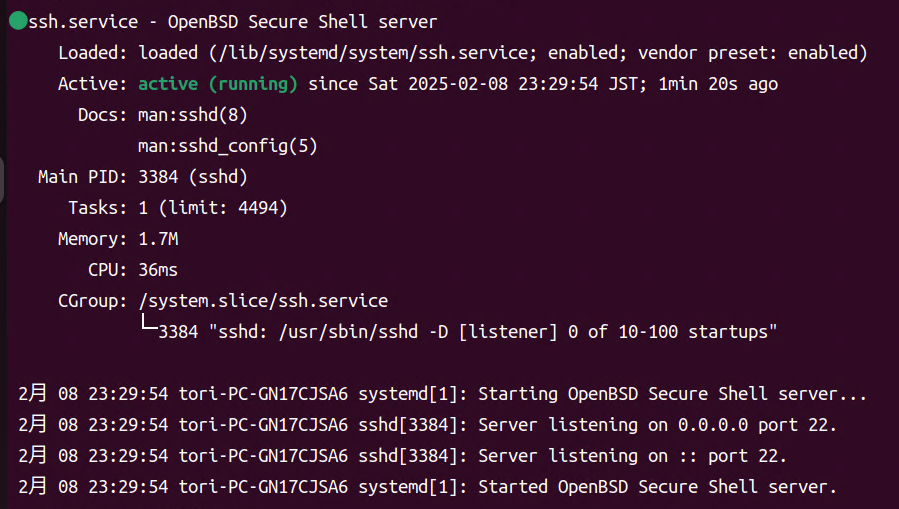
\includegraphics[width=12cm]{images/linux-server/10_2_1-status-ssh.png}
  \caption{SSHサーバーの起動確認}
\end{figure}
\begin{hosokubox}{SSHサーバーの起動}
  初期設定ではシステム起動時にSSHサーバーが自動で起動されるように設定されている。しかし、手動でSSHサーバーを起動する場合は「systemctl start ssh」コマンドを使用する。
\end{hosokubox}

\subsubsection{ポート番号の設定}
SSHサーバーはデフォルトで22番ポートを使用する。しかし、22番ポートは前述している通りウェルノウンポート番号であるため、セキュリティ上のリスクがある。そのため、一般的にポート番号を変更することが推奨される。ポート番号の変更はsshd\_configファイルを編集することで行うことができる。
\begin{attentionbox}{sshd\_configファイルのバックアップ}
  通常設定ファイルの変更の際には、設定ファイルのバックアップを取得することを推奨する。
  cpコマンドを使用し、設定ファイルのバックアップを作成しておく。
  \begin{commandbox}{設定ファイルのバックアップ}
    \verb|$ cp /etc/ssh/sshd_config /etc/ssh/sshd_config.bak|
  \end{commandbox}
\end{attentionbox}
ポート番号の変更はsshd\_configファイル内に「\#Port22」と書かれている箇所のコメントアウトを外し、ポート番号を指定することで変更することができる。
\begin{commandbox}{sshd\_configファイルの編集}
  \begin{verbatim}
  #Port 22
  Port 10022\end{verbatim}
\end{commandbox}
このままではファイアーウォールで設定されているポート番号に対して許可されていないため、ファイアーウォールの設定を変更する必要がある。
\begin{commandbox}{ファイアーウォールの設定}
  \verb|$ sudo ufw allow 10022/tcp|
\end{commandbox}
\begin{johobox}{TCPとUDP?}
  TCP(Transmission Control Protocol)とUDP(User Datagram Protocol)は、インターネットで使用される通信プロトコルである。TCPは比較的安定した通信を行いたいときに使用される。一方、UDPは速度を重視する通信を行いたいときに使用される。\\
  TCPはSSHなど通信の安全を求める。一方、UDPは動画配信などの速度を重視する通信に使用される。
\end{johobox}
\subsubsection{ログインの制限}
SSHサーバーは外部から全ての権限があるrootへのログインを制限することが推奨される。これにより、rootユーザーに対する攻撃を防ぐことができる。ログインの制限はsshd\_configファイルを編集することで行うことができる。
\begin{commandbox}{sshd\_configファイルの編集}
  \begin{verbatim}
  PermitRootLogin no    # 追加する\end{verbatim}
\end{commandbox}
また、特定のユーザーのみログインを許可する場合はAllowUsersを使用する。
\begin{commandbox}{sshd\_configファイルの編集}
  \begin{verbatim}
  AllowUsers user1 user2    # 追加する\end{verbatim}
\end{commandbox}
\subsubsection{SSHログイン}
ここまでできたら一度SSH接続を行ってみる。SSH接続の接続元(SSHサーバーを立てたPC)をサーバー、接続するPCをクライアントと呼ぶ。接続は以下のコマンドをクライアントで使用する。なお、実行にはWindowsではPoserShell、Linuxではターミナルを使用する。
\begin{commandbox}{terminal(クライアントPC)}
  \verb|$ ssh {ユーザー名}@{IPアドレス} -p {ポート番号}|
\end{commandbox}
コマンド実行後、パスワードを求められるので入力する。正しく入力された場合、SSHサーバーに接続される。
\begin{hosokubox}{初回接続}
  初回接続時にはホスト認証鍵がないため、接続時にホスト認証鍵を登録するかどうかを尋ねられる。yesを入力することでホスト認証鍵を登録することができる。
\end{hosokubox}
本書は基礎知識+Webサーバーの構築を目的とするため二段階認証についての説明は省略する。ただし、近年実際のネットワークを介してアクセスをする場合は必須とされているので、調べ、できるようになっておくべきである。
\section{基本的なサーバー管理}
\subsection{サーバー負荷}
  サーバー運用において負荷の理解は重要である。どの部分に負荷がかかっているのかを理解することでアルゴリズムの最適化やサーバースペックの見直しなどを行うことができる。サーバーの負荷を確認するにはuptimeコマンドを使用する。
  \begin{commandbox}{負荷の確認}
    \verb|$ uptime|\\
    \verb| 10:00:00 up 1 day,  1:00,  1 user,  load average: 0.00, 0.01, 0.05|
  \end{commandbox}
  uptimeコマンドの出力は稼働時間の他にload averageが表示される。load averageは1分、5分、15分の負荷平均を示している。ここでいう負荷とはCPUのコア数に対する平均負荷を示している。例えば、CPUが4コアの場合、load averageが4を超えるとCPUがフル稼働している状態となる。
\subsection{ディスクの使用状況}
ディスクの使用状況を確認するにはdfコマンドを使用する。
  \begin{commandbox}{ディスクの使用状況の確認}
    \verb|$ df -h|\\
    \verb|Filesystem      Size  Used Avail Use% Mounted on|\\
    \verb|udev            1.9G     0  1.9G   0% /dev|\\
    \verb|.......|
  \end{commandbox}
  dfコマンドの出力はファイルシステム、容量、使用、空き、使用率、マウントポイントが表示される。使用率が100\%になるとディスクがいっぱいになっているため、ディスク容量の拡張や不要なファイルの削除などを行う必要がある。
\subsection{メモリとスワップ}
メモリとスワップの使用状況を確認するにはfreeコマンドを使用する。
\begin{johobox}{スワップとは?}
  スワップはメモリが不足した場合にディスクの一部を仮想メモリとして使用する機能である。スワップが発生するとディスクアクセスが発生するため、メモリよりも遅いアクセス速度となる。そのため、スワップが発生するとパフォーマンスが低下する。 
\end{johobox}
  \begin{commandbox}{メモリとスワップの使用状況の確認}
    \verb|$ free -h|\\
    \verb|              total        used        free      shared  buff/cache   available|\\
    \verb|Mem:           1.9G        1.1G        100M        100M        700M        500M|\\
    \verb|Swap:          2.0G        100M        1.9G|
  \end{commandbox}
  freeコマンドの出力はメモリとスワップの使用状況を表示している。メモリの使用率が高い場合はプロセスの終了やメモリの増設などを行う必要がある。
\subsection{プロセスの管理}
実行中のプロセスを確認する時にはpsコマンドを使用する。実行中の全てのプロセスを確認するには以下のコマンドを実行する。
  \begin{commandbox}{プロセスの確認}
    \verb|$ ps aux|\\
    \verb|UID        PID  PPID  C STIME TTY          TIME CMD|\\
    \verb|root         1     0  0 10:00 ?        00:00:00 /sbin/init|\\
    \verb|root         2     0  0 10:00 ?        00:00:00 [kthreadd]|
  \end{commandbox}
  psコマンドの出力はプロセスの情報を表示している。プロセスの終了やプロセスの強制終了などを行う場合はkillコマンドを使用する。実際はこれ以上のプロセスが実行されているのでlessコマンドやgrepコマンドなどを使用して絞り込むことが多い。
\subsection{サービス管理}
  サービスは、OS本体から切り離し可能な特定の役割や機能を持ったサブシステムのことをいう。サービスにはログ管理やネットワーク、WebサーバーやSSHサーバーなどの各種サーバープログラムが含まれる。サービスの起動、停止、再起動はsystemctlコマンドを使用する。
  \begin{commandbox}{systemctlコマンド}
    \verb|$ sudo systemctl {サブコマンド} {サービス名}|
  \end{commandbox}
  \begin{hosokubox}{systemctlのサブコマンド}
    \begin{itemize}
      \item start : サービスの起動
      \item stop : サービスの停止
      \item restart : サービスの再起動
      \item status : サービスの状態を確認
      \item enable : サービスの自動起動を有効にする
      \item disable : サービスの自動起動を無効にする
    \end{itemize}
  \end{hosokubox}
\section{Webサーバーの構築}
ここまでサーバー操作に関する基礎を学んできた。ここからはWebサーバーの構築を行う。今回はApacheを使用したWebサーバーの構築を行う。
\begin{johobox}{Apacheについて}
  Apache HTTP Server(以下、Apache)は、Apacheソフトウェア財団が提供するオープンソースのWebサーバーソフトウェアである。1995年に開発が始まった。主な特徴として、拡張性が高く、多くのモジュールが提供されている。また、多くのOSに対応している。他にも静的コンテンツだけでなく動的なWebアプリケーションのホスティングにも対応している。
\end{johobox}
\subsection{サーバーソフトウェアのインストール}
\subsubsection{WebサーバーとWebブラウザ}
WebサーバーはHTTPプロトコルを使用してクライアントにWebページを提供するサーバーソフトウェアである。一方、WebブラウザはHTTPプロトコルを使用してWebサーバーからWebページを取得するクライアントソフトウェアである。Webブラウザとして現在有名なのが、Google Chrome、Firefox、Safari、Microsoft Edgeなどがある。
\subsection{Apache HTTP serverのインストール}
Apache HTTP serverのインストールは以下のコマンドを実行することで行うことができる。
\begin{terminalbox}
  \verb|$ sudo apt update|
  \verb|$ sudo apt -y install apache2|
\end{terminalbox}
インストール後、systemctlコマンドを使用してApache HTTP serverを起動・起動確認を行う。
\begin{terminalbox}
  \verb|$ sudo systemctl start apache2|\\
  \verb|$ sudo systemctl enable apache2|\\
  \verb|$ sudo systemctl status apache2|
\end{terminalbox}
以下のような表示がされればApache HTTP serverの起動に成功している。
\begin{figure}[H]
  \centering
  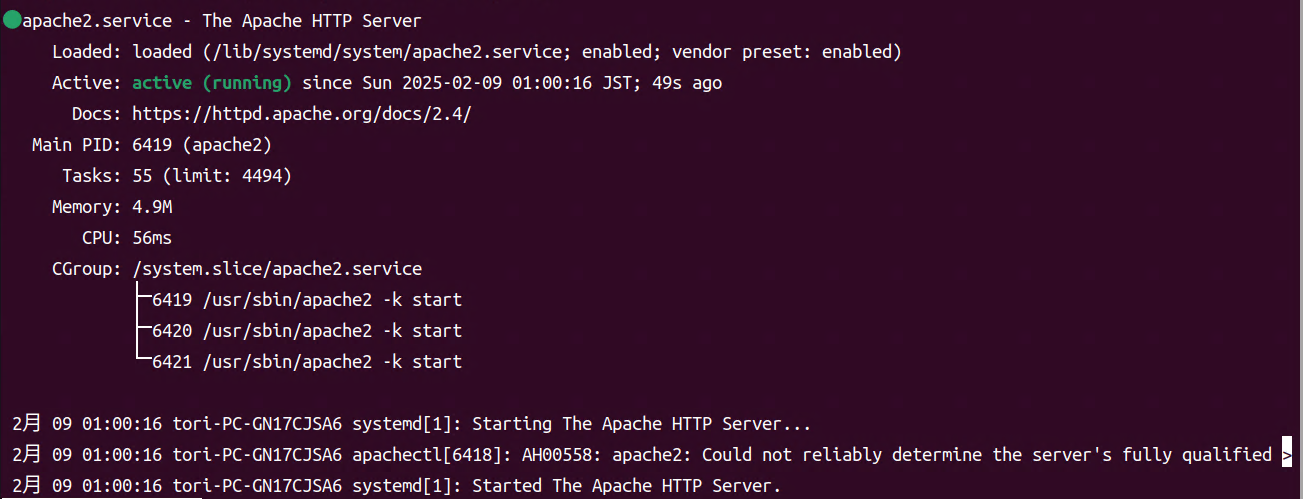
\includegraphics[width=14cm]{images/linux-server/12_3_status-apache.png}
  \caption{Apache HTTP serverの起動確認}
\end{figure}
また、ブラウザを使用してhttp://localhost/にアクセスすることでApacheのデフォルトページが表示される。
\begin{figure}[H]
  \centering
  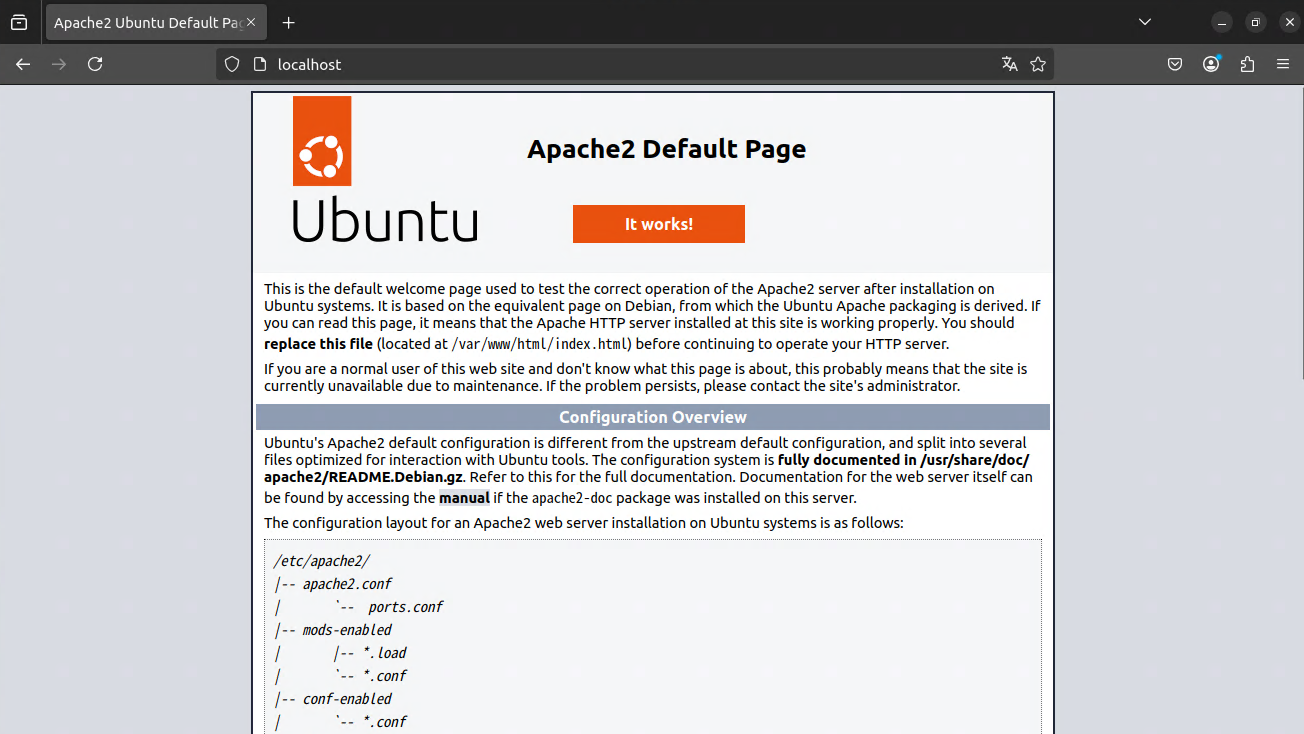
\includegraphics[width=14cm]{images/linux-server/12_3-2_welcompage.png}
  \caption{Apacheのデフォルトページ}
\end{figure}

\subsection{Apacheの設定}
ApacheはWebサーバーとして当然ながら、様々な設定を行うことができる。それらを管理するのは「/etc/apache2/apache2.conf」や「/etc/apache2/sites-available/000-default.conf」などの設定ファイルである。ここではそれらに含まれる設定について解説する。
\begin{johobox}{apache2.confファイルについて}
  apache2.confファイルはサーバー全体に適用するためのグローバル設定ファイルである。このファイルには、サーバーの設定やモジュールの読み込みなどが記述されている。
\end{johobox}
\begin{johobox}{000-default.confファイルについて}
  000-default.confファイルはサイトごとの設定ファイルである。このファイルには、サイトの設定やドキュメントルートの設定などが記述されている。サイトごとの設定ファイルのため、このファイルを変更する、もしくは、新たに仮想ホストの設定ファイルを作成することで複数のサイトを運用することができる。
\end{johobox}
\begin{attentionbox}{複数サイトの同時起動}
  Apacheは前述の通り仮想ホストによりサーバー処理を行っている。そのため1つのサーバーから複数のサイトを運用することが可能である。しかし、ローカル上で複数サイトのアクセス処理のためにはDNSサーバーによるポート転送が必要となるため今回は説明を省く。どうしても試してみたい場合は以下の参考サイトを参照するとよい。\\
  77Lifeworkベータ版, Apacheを複数起動(複数インスタンス構成)する, \url{https://www.77-lifework.com/entry/apache-multi}
\end{attentionbox}
Apacheの設定ファイルで記述可能な設定項目をディレクティブという。以下に主なディレクティブを示す。
\begin{itemize}
  \item ServerRoot : 設定ファイルなどを配置するトップディレクトリ(/etc/apache2)
  \item Listen : Apacheが受け付けるポート(80番)
  \item User : Apacheが実行されるユーザー(www-data)
  \item Group : Apacheが実行されるグループ(www-data)
  \item ServerAdmin : Apacheサーバーの管理者(webmaster@localhost)
  \item DocumentRoot : Webページを配置するディレクトリ(/var/www/html)
  \item DirectoryIndex : ディレクトリへのアクセス時に表示するファイル名(index.html)
\end{itemize}
以降では一般的なサーバーにおける変更点としてDocumentRoot、DirectoryIndexの変更を行う。また、Listenの変更を行う可能性もあるためそれについても説明する。

\subsubsection{DocumentRootとDirectoryIndexについて}
DocumentRootはWebページを配置するディレクトリを指定するディレクティブである。デフォルトでは/var/www/htmlが指定されている。ここで指定するディレクトリは「http://<サーバーIP>/」にアクセスした際に表示されるページが配置されるディレクトリである。このディレクトリの中にあるDirectoryIndexで指定したファイルが「http://<サーバーIP>/」にアクセスした際に表示されるファイルとなる。
DirectoryIndexはディレクトリへのアクセス時に表示するファイル名を指定するディレクティブである。デフォルトではindex.htmlが指定されている。このファイルが存在しない場合はindex.php、index.cgi、index.pl、index.xhtml、index.htmの順に表示される。

\subsubsection{仮想ホストの作成}
Apacheのインストール後は「000-default.conf」が仮想ホストとして設定されている。別の仮想ホストとして設定を行う。仮想ホストの設定は「/etc/apache2/sites-available/」ディレクトリ内に設定ファイルを作成する。ファイル名は任意であるが、一般的には「サイト名.conf」とする。ここでは「.conf」とする。
\begin{hosokubox}{仮想ホストの設定について}
  デフォルトで用意されているファイルを使用する場合は「000-default.conf」編集して使用してもよい。また、設定をゼロから記述するのが大変な場合はcpコマンドを使用する方法などもある。
\end{hosokubox}
\begin{commandbox}{terminal:仮想ホストの設定ファイルの作成}
  \begin{verbatim}
  $ sudo touch /etc/apache2/sites-available/{ファイル名}.conf\end{verbatim}
\end{commandbox}
作成したファイルに以下の最小構成の設定を記述する。DocumentRootとDirectoryIndexは先ほど説明したとおりに設定を行う。
\begin{commandbox}{/etc/apache2/sites-available/{ファイル名}.conf}
  \begin{verbatim}
  <VirtualHost *:80>
    ServerAdmin webmaster@localhost
    DocumentRoot {ディレクトリ名}
    DirectoryIndex {ファイル名}
    ErrorLog ${APACHE_LOG_DIR}/error.log
    CustomLog ${APACHE_LOG_DIR}/access.log combined
  </VirtualHost>\end{verbatim}
\end{commandbox}
\begin{hosokubox}{APACHE\_LOG\_DIRについて}
  APACHE\_LOG\_DIRはApacheのログファイルを保存するディレクトリを指定する環境変数である。デフォルトでは/var/log/apache2に設定されている。この変数の変更にはapache2.confファイルを編集する必要がある。
\end{hosokubox}
変更後、DocumentRootに指定したディレクトリがない場合は作成し、DirectoryIndexを作成する。
\begin{commandbox}{terminal:ディレクトリの作成}
  \begin{verbatim}
  $ sudo mkdir {ディレクトリ名}
  $ sudo touch {ディレクトリ名}/{ファイル名}\end{verbatim}
\end{commandbox}
作成後、設定ファイルの有効化にはa2ensiteコマンドを使用し、仮想ホストの有効化を行う必要がある。
\begin{commandbox}{terminal:仮想ホストの有効化}
  \begin{verbatim}
  $ sudo a2ensite {ファイル名}.conf
  $ sudo systemctl restart apache2\end{verbatim}
\end{commandbox}
Apacheの再起動後systemctlコマンドを使用してApacheの状態を確認する。(sudo systemctl status apache2)。起動が確認出来たら、ブラウザを使用してhttp://localhost/にアクセスすることで新たに作成した仮想ホストのページが表示される。
\begin{attentionbox}{仮想ホストの無効化}
  仮想ホストの無効化を行わない場合、localhostにアクセスした際前述で作成したページにアクセスできない場合がある。また、サーバーへの負荷がかかってしまう。そのため、不要な仮想ホストの無効化を行うことが必要である。一方、仮想ホストを同時に立てる場合は別の手段となる。
  \begin{commandbox}{仮想ホストの無効化}
    \verb|$ sudo a2dissite {ファイル名}.conf|\\
    \verb|$ sudo systemctl restart apache2|
  \end{commandbox}
\end{attentionbox}
\begin{figure}[H]
  \centering
  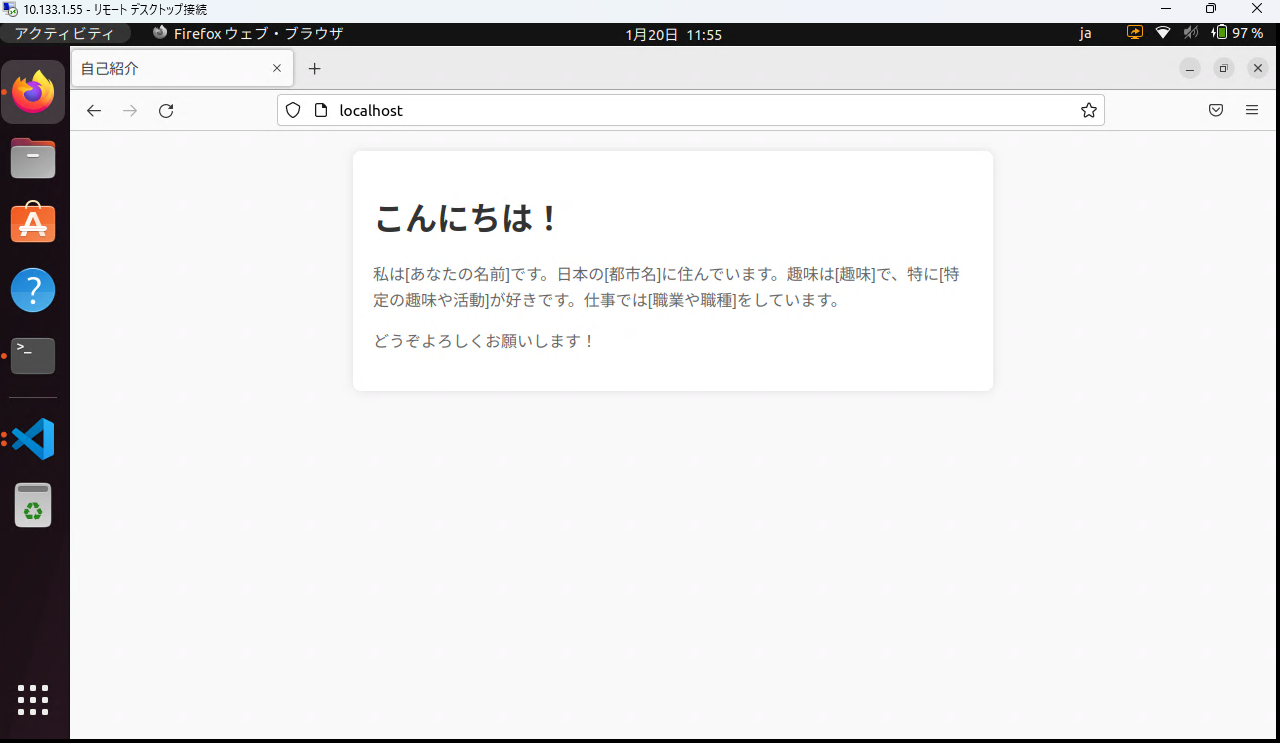
\includegraphics[width=14cm]{images/linux-server/12_3_2-1apache-test-conf.png}
  \caption{新たに作成した仮想ホストのページ}
\end{figure}
\subsubsection{ポートの変更}
ポートの変更には「Listen」ディレクティブを使用する。デフォルトでは80番ポートが指定されている。ポートの変更は以下のように行う。
\begin{commandbox}{/etc/apache2/ports.conf}
  \begin{verbatim}
  Listen 8080\end{verbatim}
\end{commandbox}
変更後、Apacheの再起動を行うことでポートの変更が適用される。
\subsection{ファイアウオールの設定}
SSHの設定の際さらっと出てきていたがここでもファイアウォールの設定を行う。
\begin{johobox}{ファイアウォールについて}
  ファイアウォールは、ネットワーク上で通信を制御するための装置やソフトウェアのことをいう。ファイアウォールは、外部からの不正アクセスや攻撃を防ぐために使用される。この機能はWindowsやmacOSなどのOSにも搭載されている。今回はufwを使用してファイアウォールの設定を行う。ufwはUncomplicated Firewallの略で、比較的簡単に設定を行うことができる。
\end{johobox}
\begin{commandbox}{ファイアウォールの有効化}
  \begin{verbatim}
  $ sudo ufw enable
  $ sudo ufw allow Apache
  $ sudo ufw status\end{verbatim}
\end{commandbox}
\begin{hosokubox}{ポート開放について}
  ファイアウォールの設定においては、ポートの開放が重要である。ポートの開放を行わない場合、外部からのアクセスが拒否されるため、Webサーバーにアクセスすることができない。ポートの開放は「sudo ufw allow ポート番号」コマンドを使用して行う。
\end{hosokubox}
\begin{commandbox}{ポート開放:80と8080の開放}
  \begin{verbatim}
  $ sudo ufw allow 80/tcp
  $ sudo ufw allow 8080/tcp\end{verbatim}
\end{commandbox}

\subsection{パスワード認証}
通常はアクセスした人全員がWebページの閲覧が可能である。しかし、特定のユーザーのみ閲覧可能なページの作成も可能となっている。それらの実現には一般的にユーザー名、パスワードによる認証が用いられる。その中で最も簡単な認証方法として基本認証がある。基本認証はユーザー名とパスワードを使用して認証を行う方法である。基本認証はApacheの設定ファイルに記述することで設定を行うことができる。
\begin{hosokubox}{apache2-utilsについて}
  認証を行うためのパッケージであるapache2-utilsは最新バージョンの場合インストールに含まれている。しかし、環境やバージョンなどによって含まれない場合もあるため念のためインストールをすることを推奨する。
\end{hosokubox}
\begin{commandbox}{apache2-utilsのインストール}
  \verb|$ sudo apt install apache2-utils|
\end{commandbox}
\subsubsection{htpasswdの作成}
インストールした後、apache2-utilsに含まれるhtpasswdコマンドを使用してユーザー名とパスワードを記述したファイルを作成する。初回の登録時には「-c」オプションを使用する。
\begin{commandbox}{htpasswdの作成}
  \begin{verbatim}
  $ sudo htpasswd -c /etc/apache2/.htpasswd {ユーザー名}  # 初回のみ
  $ sudo htpasswd /etc/apache2/.htpasswd {ユーザー名} # 2回目以降
  New password: {パスワード}
  Re-type new password: {パスワード}\end{verbatim}
\end{commandbox}
ユーザー登録の完了後、認証を利用する仮想ホストの設定ファイルに以下の設定を追加する。
\begin{commandbox}{/etc/apache2/sites-available/{ファイル名}.conf}
  \begin{verbatim}
  <Directory {認証を利用したいディレクトリパス}>
    AuthType Basic
    AuthName "Restricted Content"
    AuthUserFile /etc/apache2/.htpasswd
    Require valid-user
  </Directory>\end{verbatim}
\end{commandbox}
設定後、Apacheの再起動を行うことで設定が適用される。
\begin{attentionbox}{認証を利用したいディレクトリについて}
  指定したディレクトリ以下にあるもの全てに認証がかかるようになるため注意が必要である。
\end{attentionbox}
\subsection{アクセスログ}
アクセスログはWebサーバーにアクセスした際の情報を記録するログファイルである。これが読めるようになることでサーバーの状況を理解し、不正アクセスなどがあった際、おかしな部分として気づくことができる。Apacheのアクセスログのデフォルトは/var/log/apache2/access.logである。アクセスログから読み取れるといいものをいかに挙げる。
\begin{itemize}
  \item リクエストさいれたURL
  \item アクセス元のIPアドレス
  \item ユーザーエージェント
  \item ステータスコード
  \item リクエストの日時
\end{itemize}
アクセスログの設定は「/etc/apache2/apache2.conf」ファイルに記述されている。以下にアクセスログの設定例を示す。
\begin{commandbox}{アクセスログの例}
  \begin{verbatim}
::1 # アクセス元のIPアドレス(ローカルのため::1)
- # リモートユーザー名
  [10/Feb/2025:22:30:31 +0900]  # リクエストの日時
  "GET / HTTP/1.1" 200 2170 "-" "Mozilla/5.0  # リクエストの内容
  (Windows NT 10.0; Win64; x64)   # ユーザーエージェント
  AppleWebKit/537.36 (KHTML, like Gecko)  # ユーザーエージェント
  Chrome/132.0.0.0 Safari/537.36" # アクセスブラウザ\end{verbatim}
\end{commandbox}
アクセスログの例をまとめると次のようになる。
\begin{itemize}
  \item アクセス元のIPアドレス(::1)
  \item リモートユーザー名(-)
  \item リクエストの日時(10/Feb/2025:22:30:31 +0900)
  \item リクエストの内容(GET / HTTP/1.1)
  \item ステータスコード(200)
  \item アクセスしたウエブブラウザ(Chrome)
\end{itemize}
\begin{johobox}{ステータスコード}
  いくつかのステータスコードを以下に示す。
  \begin{itemize}
    \item 200 : OK(リクエストが成功した)
    \item 401 : Unauthorized(認証が必要)
    \item 403 : Forbidden(アクセスが拒否された)
    \item 404 : Not Found(リクエストされたリソースが見つからない)
    \item 500 : Internal Server Error(サーバー内部のエラー)
  \end{itemize}
\end{johobox}
\subsection{エラーログ}
サーバーを管理する上で重要なものとしてエラーログも挙げられる。これにはサーバー運用時に発生したエラーの情報が記録されている。Apacheのエラーログのデフォルトは/var/log/apache2/error.logである。ただしエラーログについては様々なものがあるため、適宜対話型AIなどを用いて解決することがよいと思われる。そのためここでの説明は省略する。
\newpage
\section{参考リンク}
Ubuntuについて\\
RedHat, Linuxとは, \url{https://www.redhat.com/ja/topics/linux/what-is-linux}\\
Canonical Ubuntu, Ubutu \url{https://jp.ubuntu.com}\\
エンジニアの入口, 【初心者でもわかる】Ubuntuのインストール方法まとめ, \url{https://eng-entrance.com/ubuntu-install}\\
金子邦彦研究室, Ubuntu 24.04のインストールガイド \url{https://www.kkaneko.jp/tools/ubuntu/ubuntudesktop.html}\\
Quita, @yuta\_931214(yuta kimura), 【初学者向け】Linuxのファイル構造についてまとめてみた, \url{https://qiita.com/yuta_931214/items/7cd5df422e05cf07c2f8}
\\\\
使用PC\\
リコレ!, Gateway NE132 NE132-F14P 〔Windows 10〕, \url{https://used.sofmap.com/r/item/2133024911019}\\
\\\\
便利機能インストール\\
Quita, @takuya66520126A(takuya), ubuntuで日本語入力に変更する方法, \url{https://qiita.com/takuya66520126/items/8bb760bf99c4e25364e3}\\
Quita, @tommy\_g, UbuntuにVimをインストールする \url{https://qiita.com/tommy_g/items/3ad4b26ccb4893f2760e}\\
Quita, @to-fmak(Wenzhang), Linuxの面白いコマンド9選 \url{https://qiita.com/to-fmak/items/ea345839f394db781bd0}\\
Zenn, koki, cmatrix コマンドでターミナルに文字を降らせる \url{https://zenn.dev/kou_pg_0131/articles/cmatrix-introduction}\\
\\
ネットワーク関連\\
Quita, @pe-ta(ペーた), ifconfigの出力結果に書いてあること \url{https://qiita.com/pe-ta/items/aff8db72530c6baa11b2}\\
Quita, @kooohei(Kohei Yamada), 静的ルーティングの設定 - Linux \url{https://qiita.com/kooohei/items/b0931ae210911cc52adc}\\
\\
ユーザー管理\\
Quita, @3062\_in\_zamud(3062.\_zamud), [chown]ファイルやディレクトリの所有者を変更する方法 \url{https://qiita.com/3062_in_zamud/items/d93770016e7d931a5983}\\
\\
Apache\\
Quita, @Apache \url{https://qiita.com/tags/apache}\\
77Lifeworkベータ版, Apacheを複数起動(複数インスタンスを構成)する, \url{https://www.77-lifework.com/entry/apache-multi}\\
JavaDrive, Listenディレクティブ:リクエストを受け付けるポート番号, \url{https://www.javadrive.jp/apache/ini/index3.html}
Apache, Apache HTTP サーバ バージョン 2.2 バーチャルホストの例, \url{https://httpd.apache.org/docs/2.2/ja/vhosts/examples.html}\\
InfoAcademy, Apacheのログの場所は?ログの場所を設定する方法について詳しく解説【Linux】, \url{https://engineer-ninaritai.com/apache-log-directory/}\\









\newpage
\section{終わりに}
サーバー構築お疲れさまでした。ここまでLinuxの基礎的な部分から少し踏み込んだ部分も含めて解説をしました。筆者もそうですが1度するだけでは覚えていません。実際に同じように立てたい時が来た時にまた見返せばいいのです。\\

反省として画像をもっと入れるべきだと思っております。改訂版が出た暁にはさらに見やすいものを心がけるつもりです。\\
それでは今後とも楽しいLinuxライフを!


\end{document}

